
\chapter{Phylogenetic distribution}
\label{phylo}

Overall my results support the identification of tenrecs as a Family with high morphological diversity compared to golden moles (Chapter \ref{chap:disparity}). These results were most conclusive when I sub-sampled the \textit{Microgale} tenrecs to account for the high morphological diversity within this Genus (Chapter \ref{chap:disparity}).

It was not necessary to sub-sample my golden mole species because the specimens I measured are spread across the phylogeny of this clade: there are no species-rich, clustered golden mole Genera similar to the \textit{Microgale} tenrec Genus (Figure \ref{fig:phylo}).

There is some debate surrounding phylogenetic relatedness within the tenrec and golden mole clades. Detailed molecular studies have established well-supported phylogenetic trees for tenrecs \citep{Poux2008, Asher2006} and golden moles \citep{Asher2010} but there is still disagreement about the resolution of some polytomies within these clades. Furthermore, recent analyses have demonstrated that there are many possible ways in which polytomies can be resolved within mammal phylogenies, including tenrecs and golden moles \citep{Kuhn2011}. Therefore, there are no single consensus trees available for either tenrecs or golden moles.

As an example, Figure \ref{fig:phylo} depicts one combined tenrec and golden mole phylogeny extracted from a distribution of possible polytomy resolutions \citep{Kuhn2011} within a mammalian supertree \citep{Fritz2009, Bininda2007}. This example is for illustrative purposes only, more detailed consideration of the effects of branching patterns on calculations of morphological diversity would be based on a distribution of phylogenies instead of just one tree. The phylogeny is derived from species included in Wilson and Reeder's Mammal Species of the World \citeyearpar{Wilson2005}. Six tenrec species (all belonging to the \textit{Microgale} Genus) and two golden mole species (\textit{Eremitalpa grandi} and \textit{Cryptochloris wintoni}) are not included in Wilson and Reeder's taxonomy. I added these species to the tree using the functions \texttt{add.species.to.genus} (for the missing \textit{Microgale}) and \texttt{findMRCA} (for the missing golden moles) from the R package phytools \citep{Revell2012}. Code for all of my analyses is available on GitHub \citep{Finlay2015c}. 

In Figure \ref{fig:phylo}, species which were not included in my morphological data are highlighted in bold. Aside from the \textit{Neamblysomus} Genus, my morphological data included representatives of all other golden mole Genera. Therefore, my golden mole specimens are not a phylogenetically clustered sub-sample of the Family so there is no reason to expect that they would have lower morphological diversity than tenrecs simply as an artefact of branching pattern. 
Furthermore, Figure \ref{fig:phylo} shows how the \textit{Microgale} tenrecs are more species-rich and phylogenetically clustered than the rest of the Family, justifying my choice to sub-sample this Genus for further investigations of morphological diversity (Chapter \ref{chap:disparity}).



 
%------------------------------------------
\begin{landscape}
\begin{figure}[h] 
  \centering
  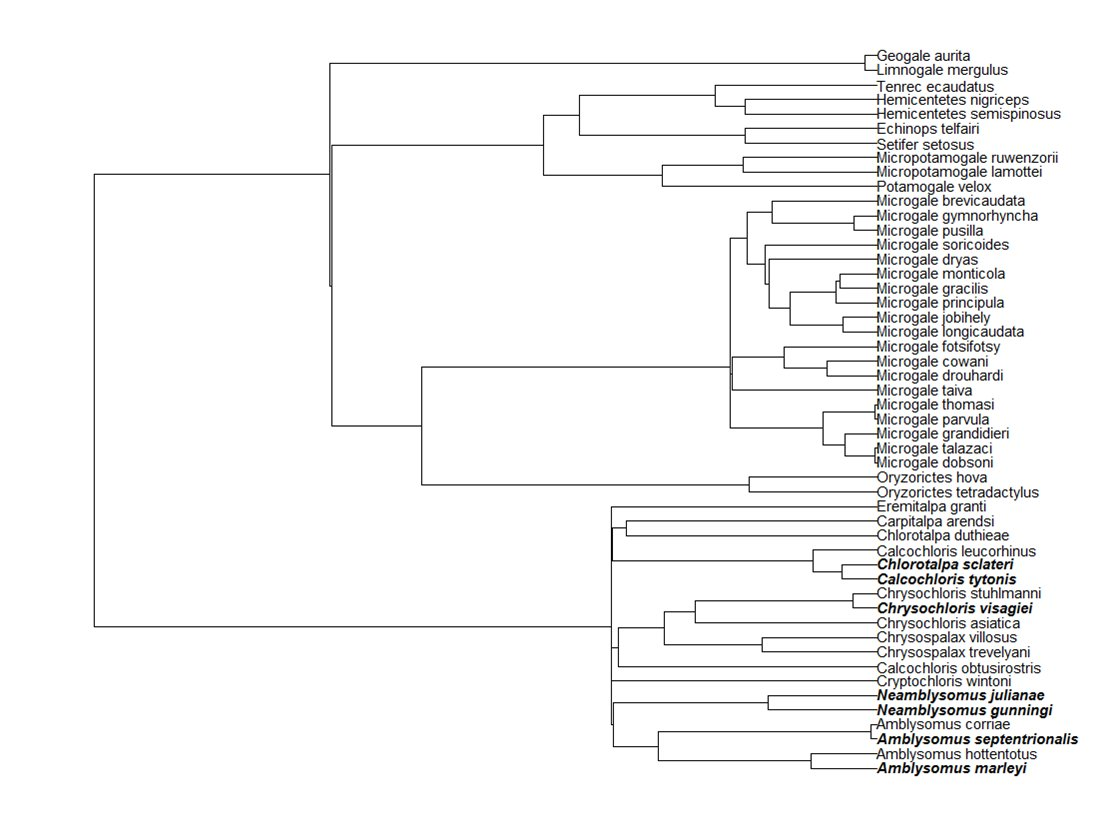
\includegraphics[width=\textwidth, height=\textheight, keepaspectratio=true]{Appendix/tc+gm_phylo.jpg}
    \caption[Example phylogeny of tenrecs and golden moles]
    {Example phylogeny of tenrecs and golden moles (one tree from a distribution of the different possible ways in which polytomies may be resolved \citep{Kuhn2011}). Golden mole species which were not represented in my morphological data are highlighted in bold. }
  \label{fig:phylo}
  \end{figure}
 \end{landscape}